\chapter{Hubble design specifics and results}\label{chap:hubble}
\thispagestyle{fancy} %Resets custom page number location on first chapter page

\section{Model and setup}\label{sec:hubble}

As an example of a 2-mirror system, we model a Ritchey--Chr{\'e}tien-style Hubble Space Telescope in Optiland (Figure~\ref{fig:hubble}; EPD\,$=$\,2400\,mm, $\lambda=0.55\,\mu\mathrm{m}$) with misalignments applied only to the secondary mirror. The five degrees of freedom are: decenter $sdx$, $sdy$ and despace $sdz$ (microns), and tilts $stx$, $sty$ (degree). Normalized field coordinates are relative to a maximum field angle of $0.038^{\circ}$.

PSFs are computed with \bashinline{MMDFTPSF} using the default \bashinline{num_rays=128}, which samples the pupil with $64\times64$ rays and produces a $256\times256$ image (Table~\ref{tab:psf_sampling}); the central $64\times64$ pixels are retained and projected onto 15 circular-Bessel basis functions (Figure~\ref{fig:bessel_basis}). The synthetic observations are computed from PSFs with additive Gaussian noise ($\sigma=0.01$ per pixel, in PSF intensity units, or $0.01\%$ of the ideal peak), while forward-model PSFs in the likelihood are noise free. Synthetic truth coefficients are stored at five normalized fields: $(0,0)$, $(1,0)$, $(0,1)$, $(1,1)$, and $(-1,-1)$. For each field, a $15\times15$ covariance matrix is estimated from $10^4$ noise-free Monte Carlo draws of $\boldsymbol{\theta}$ under zero-mean Gaussian perturbations ($\sigma=100\,\mu\mathrm{m}$ on translations, $\sigma=0.167$ degrees on tilts), with each draw rounded to two decimal places.

\begin{figure}
    \centering
    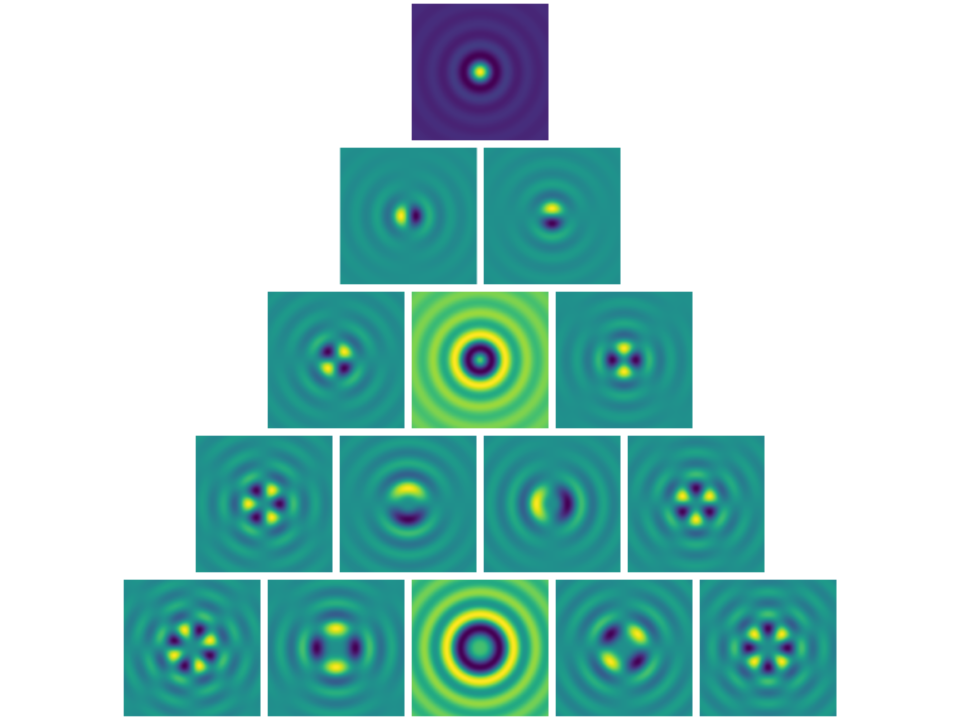
\includegraphics[width=0.75\textwidth]{figures/circular_bessel_basis.png}
    \caption[The circular-Bessel basis functions used for the Hubble PSFs.]{The 15 circular-Bessel basis functions used for the Hubble PSFs, $J_{n+1}(2\pi\rho)\cos(m\phi)/\rho$ and $J_{n+1}(2\pi\rho)\sin(m\phi)/\rho$, arranged by radial order $n=0$--4 from top to bottom. Up to a constant factor, each is the Fourier transform of the Zernike mode in the same position of Figure~\ref{fig:zernike_basis}~\citep{Noll1976}. Each panel has its own color scale.}
    \label{fig:bessel_basis}
\end{figure}

Uniform priors on the unit cube map to $\pm200\,\mu\mathrm{m}$ on $(sdx,sdy,sdz)$ and $\pm0.167$ degrees on $(stx,sty)$; samples from the prior transform are rounded to $0.01\,\mu\mathrm{m}$ and $0.01$ degrees. Nautilus runs with \bashinline{n_dim=5}. In our completed benchmark, the sampler performed 44\,000 likelihood evaluations with $\ln\mathcal{Z}\approx +62.3$ and $N_{\mathrm{eff}}\approx 1.43\times 10^4$. The weighted median of the last 100 posterior samples provides the starting point for DE.

The DE objective is the unweighted sum of squared coefficient residuals over all five fields, $\sum_{f\in\mathcal{F}}\sum_{k=1}^{15}[c_{f,k}(\boldsymbol{\theta})-c_{f,k,\mathrm{obs}}]^2$, minimized with \bashinline{tol=1e-12}; the run reached its limit of 2000 generations, and L-BFGS-B polishing left the solution unchanged. Nautilus constrains $sdz$ and the tilts but leaves $sdx$ and $sdy$ broad (Section~\ref{sec:hubble_results}), so DE must locate the decenters within wide posterior-derived bounds.

\begin{figure}
    \centering
    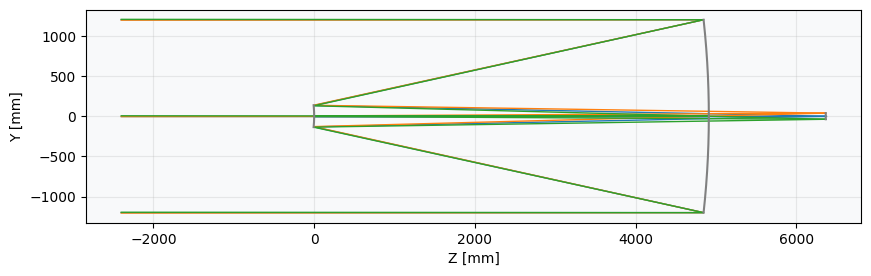
\includegraphics[width=\columnwidth]{figures/hubble.png}
    \caption{Optiland ray trace of the Hubble model. Likelihood evaluation uses circular-Bessel coefficients at five field coordinates (see text).}
    \label{fig:hubble}
\end{figure}

\section{Results}\label{sec:hubble_results}

One realization with noisy observations was injected with translations $(sdx,sdy,sdz)=(52.22,\,-113.86,\,38.99)\,\mu\mathrm{m}$ and tilts $(stx,sty)=(0.13,\,-0.04)$ degrees. Nautilus ($\ln\mathcal{Z}\approx +62.3$) tightly constrained both tilts and, more loosely, $sdz$, but left $sdx$ and $sdy$ unconstrained: their marginals in Figure~\ref{fig:hubble_corner} are close to flat across the $\pm200\,\mu\mathrm{m}$ prior. The weighted median of the final 100 posterior samples, used to start DE, was $(51.06,\allowbreak\,-0.66,\allowbreak\,39.60,\allowbreak\,0.12,\allowbreak\,-0.04)$, and the corresponding 2.1\%--97.9\% DE bounds span $\approx 327\,\mu\mathrm{m}$ on $sdx$ and $\approx 378\,\mu\mathrm{m}$ on $sdy$. After 2000 generations, differential evolution reached $\mathbf{c}=(53.77,\allowbreak\,-110.04,\allowbreak\,39.07,\allowbreak\,0.1296,\allowbreak\,-0.0398)$ with objective $6.2\times10^{-5}$, leaving residuals of $1.55$, $3.82$ and $0.08\,\mu\mathrm{m}$ on $sdx$, $sdy$ and $sdz$ and $\lesssim 4\times10^{-4}$ degrees on the tilts (Table~\ref{tab:hubble}). The objective came within 4\% of this value by generation 30 and was essentially flat afterwards. The remaining cost is set by the observation noise: the expected sum of squared coefficient noise over the five fields, less the five fitted parameters, is $\approx 5.3\times10^{-5}$ (Section~\ref{sec:noise_de}).

\begin{figure}
    \centering
    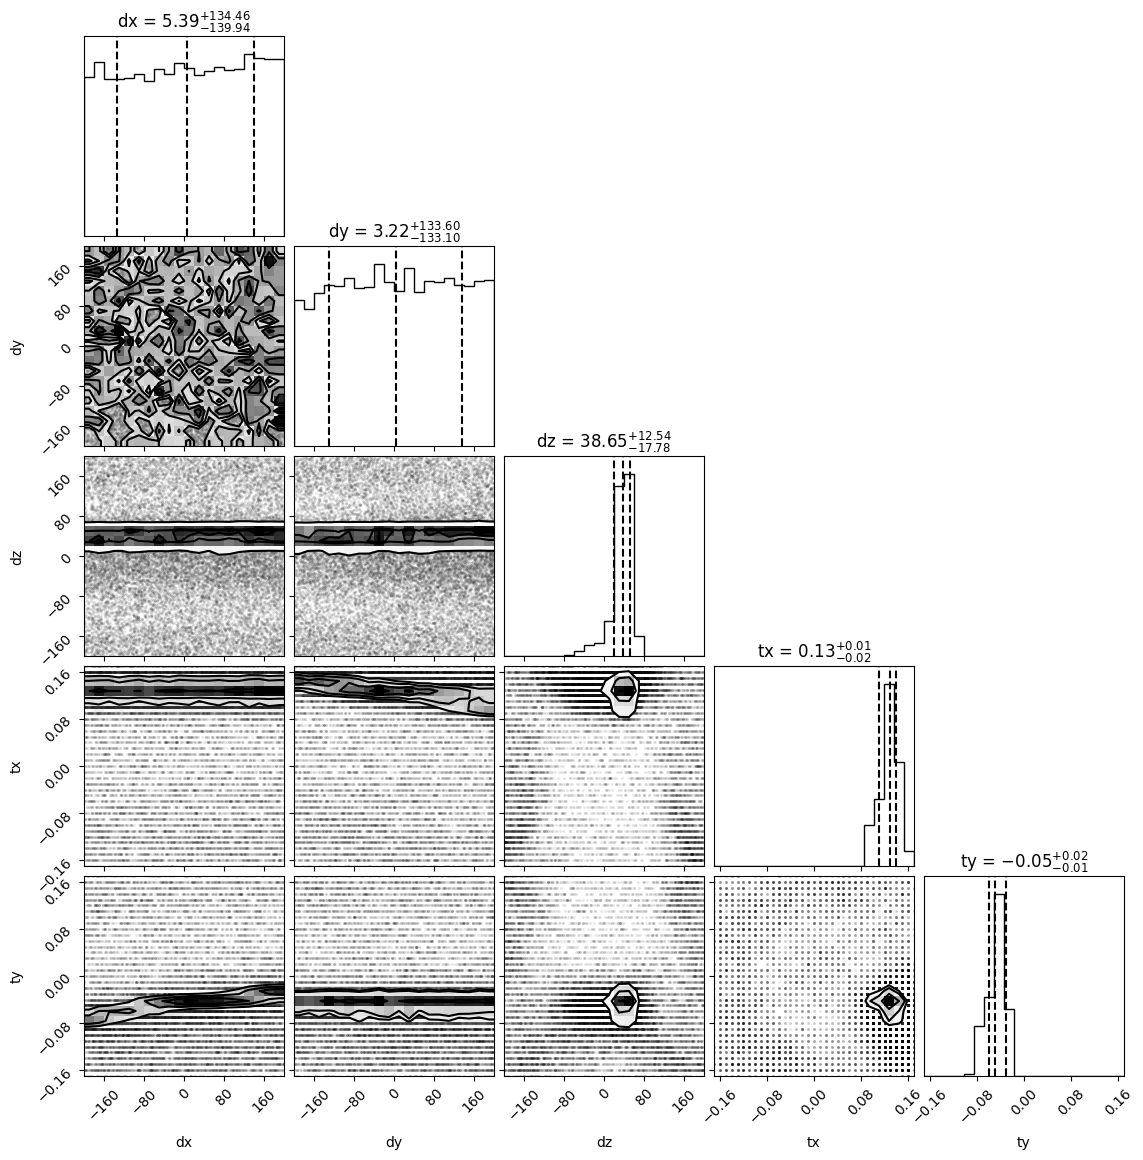
\includegraphics[width=\columnwidth]{figures/hubbletilus.png}
    \caption{Nautilus posterior corner plot for the five secondary-misalignment parameters of the Hubble model (axes labelled $dx$, $dy$, $dz$, $tx$, $ty$ correspond to $sdx$, $sdy$, $sdz$, $stx$, $sty$). Titles give the full-posterior marginal medians.}
    \label{fig:hubble_corner}
\end{figure}

\begin{figure*}
    \centering
    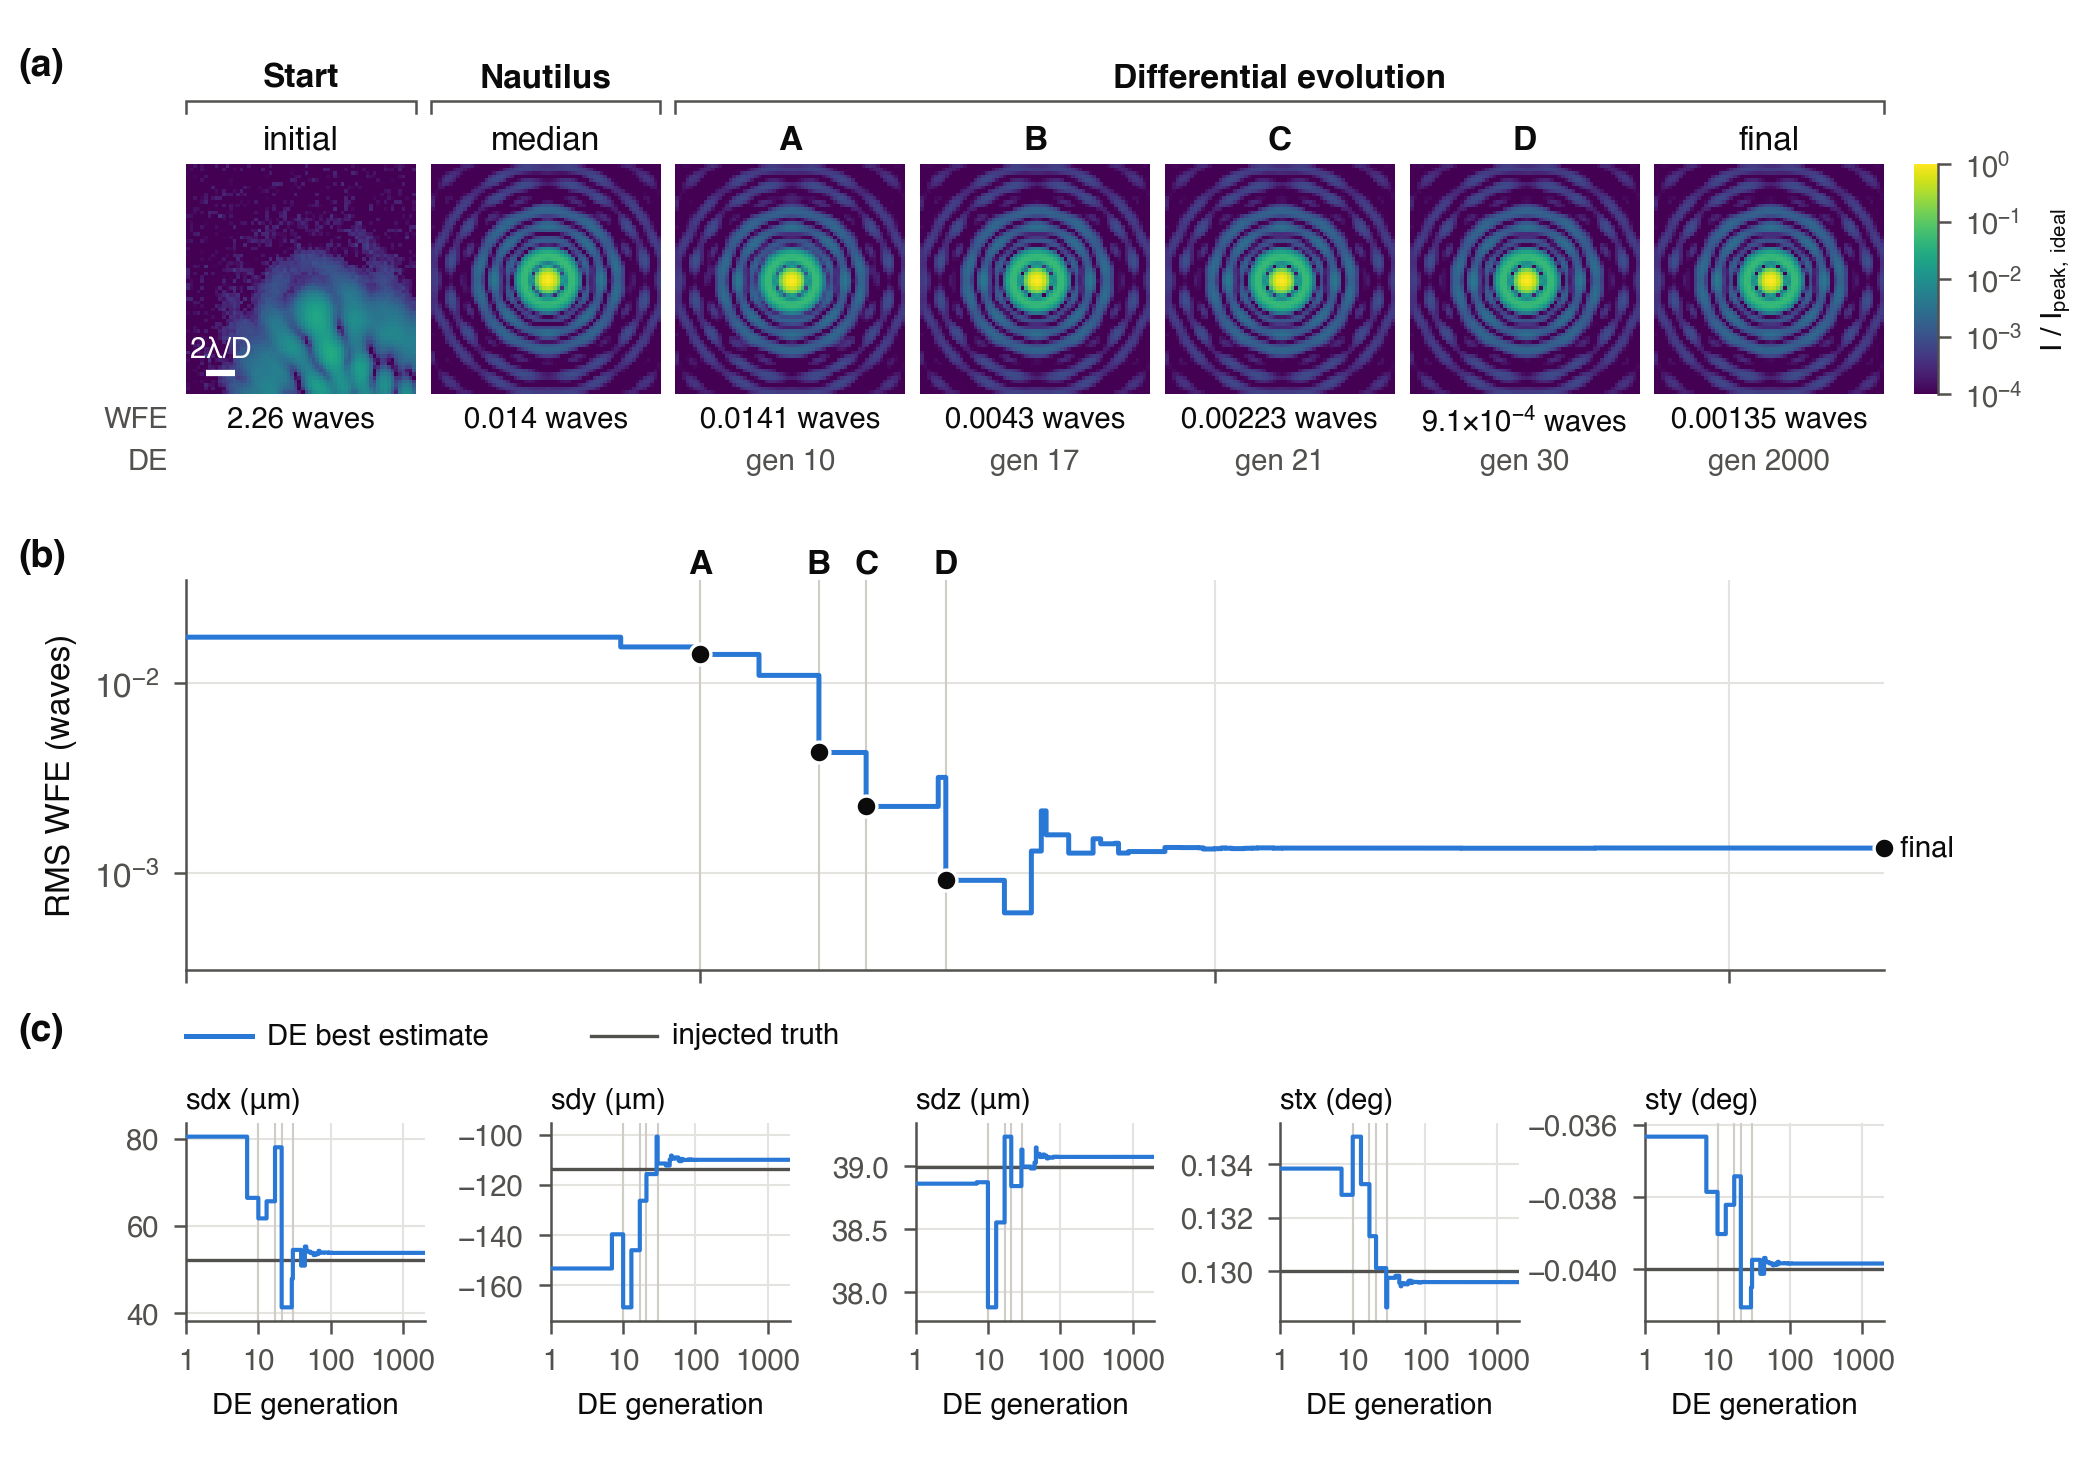
\includegraphics[width=\textwidth]{figures/psf_progression.png}
    \caption{Hubble benchmark with noisy PSFs: on-axis PSF and RMS wavefront error (WFE; the on-axis OPD RMS quoted in the text) as the alignment is refined. (a) PSFs for the uncorrected system (the observed PSF, with Gaussian noise of $\sigma=0.01\%$ of the ideal peak), the Nautilus starting point (median of the final 100 posterior samples), DE solutions at generations 10, 17, 21 and 30 (A--D) and the DE solution after 2000 generations (final). (b) RMS WFE of the DE best estimate versus generation. (c) DE best estimate of each secondary-mirror parameter versus generation, with the injected truth.}
    \label{fig:psf_prog}
\end{figure*}

\begin{figure*}
    \centering
    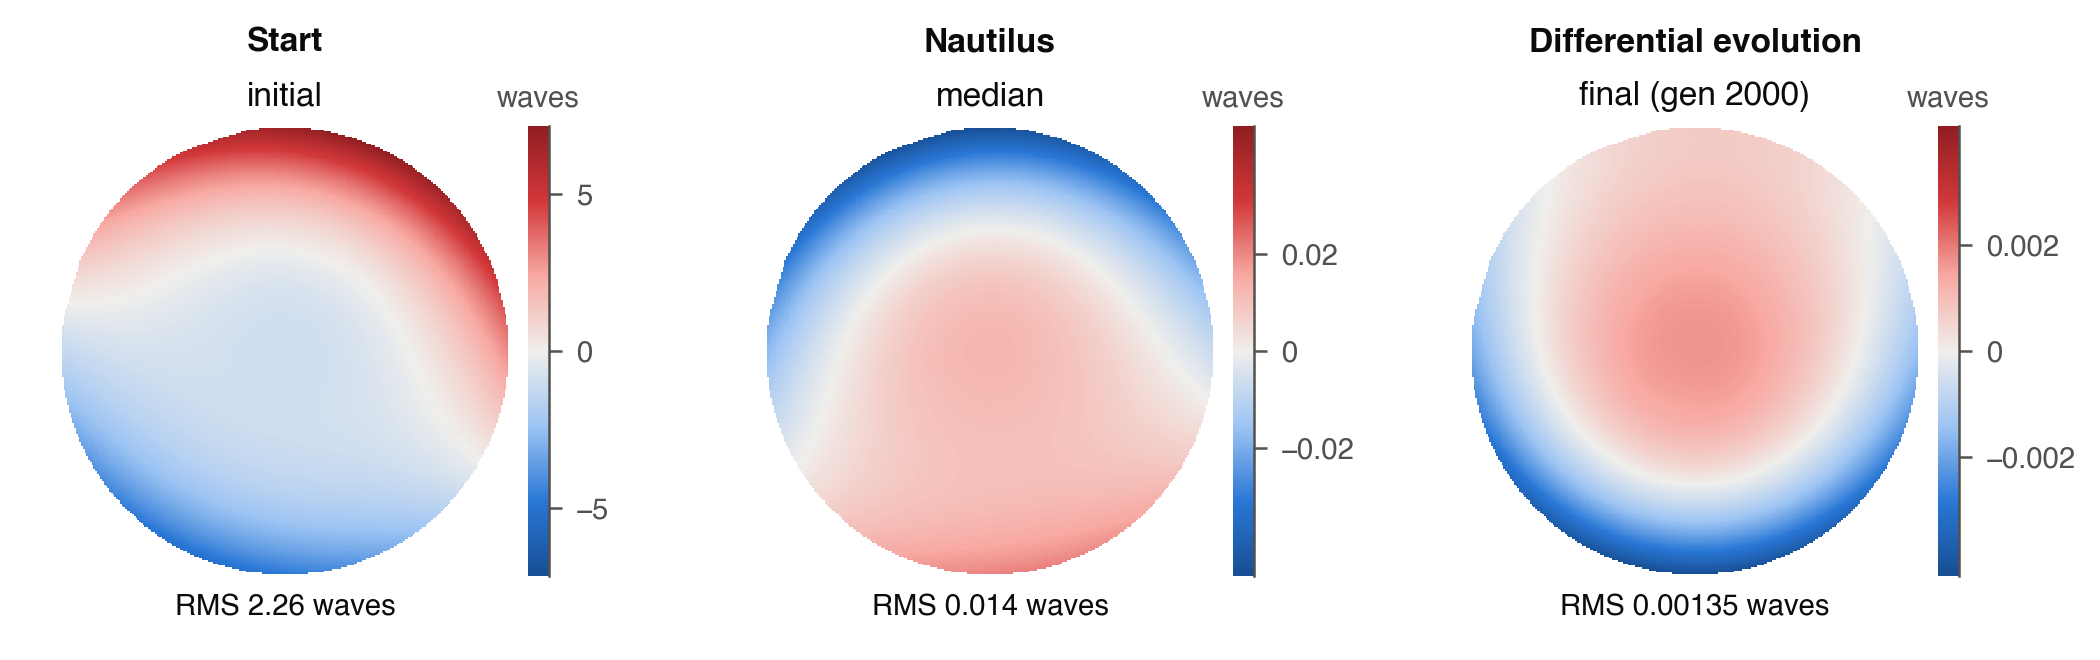
\includegraphics[width=\textwidth]{figures/hubble_opd.png}
    \caption{Residual on-axis OPD maps of the Hubble model: the difference between the nominal design and the system with residual misalignment $\boldsymbol{\theta}_{\mathrm{true}}-\mathbf{c}$, for the uncorrected system, the Nautilus starting point and the DE solution after 2000 generations. Piston is removed and tilt is retained, as in the quoted RMS WFE. Each panel has its own symmetric color scale in waves, with zero in gray. By variance, the final residual is 57\% defocus and 39\% tilt.}
    \label{fig:hubble_opd}
\end{figure*}

\begin{table}
\centering
\caption[Hubble secondary: injected truth and DE-recovered misalignment.]{Hubble secondary: injected truth and DE-recovered misalignment (noisy PSFs, $\sigma=0.01\%$ of the ideal peak; after 2000 DE generations and L-BFGS-B polishing). Tilts are in degrees.}
\label{tab:hubble}
\begin{tabular}{llll}
\hline
\textbf{Parameter} & \textbf{True value} & \textbf{Recovered (DE)} & \textbf{Units} \\
\hline
sdx & $52.22$  & $53.77$  & $\mu$m \\
sdy & $-113.86$ & $-110.04$ & $\mu$m \\
sdz & $38.99$  & $39.07$  & $\mu$m \\
stx & $0.13$   & $0.1296$   & degree \\
sty & $-0.04$  & $-0.0398$  & degree \\
\hline
\end{tabular}
\end{table}

With no correction, on-axis OPD RMS is $\sim 2.26$ waves. Using the DE starting point (the median of the final 100 posterior samples) alone reduces this to $\sim 0.014$ waves. After DE refinement, on-axis OPD RMS falls to $\sim 1.3\times 10^{-3}$ waves. Because the objective is limited by noise, the on-axis OPD RMS does not decrease monotonically: it reaches $6\times10^{-4}$ waves at generation 39 before settling at $1.3\times10^{-3}$ waves. Figure~\ref{fig:hubble_corner} shows posterior marginals for all five secondary misalignments, and Figure~\ref{fig:psf_prog} shows the on-axis PSF and RMS wavefront error at each stage of the refinement. The residual OPD maps (Figure~\ref{fig:hubble_opd}) show what remains: the final residual is mostly defocus (57\% of the variance) and tilt (39\%), the low-order aberrations left by the small despace error and by the decenter--tilt trade-off described in Section~\ref{sec:noise_de}.